\documentclass[12pt]{article}
\usepackage{bookmark}
\usepackage{graphicx}
\usepackage[a4paper]{geometry}
\usepackage{amsmath}
\usepackage{amssymb}
\usepackage{float}
\newcommand{\dotp}{{\boldsymbol \cdot}}
\begin{document}
\title{Notes on Multivariable Calculus}
\author{BatuCem}
\date{\today}
\maketitle
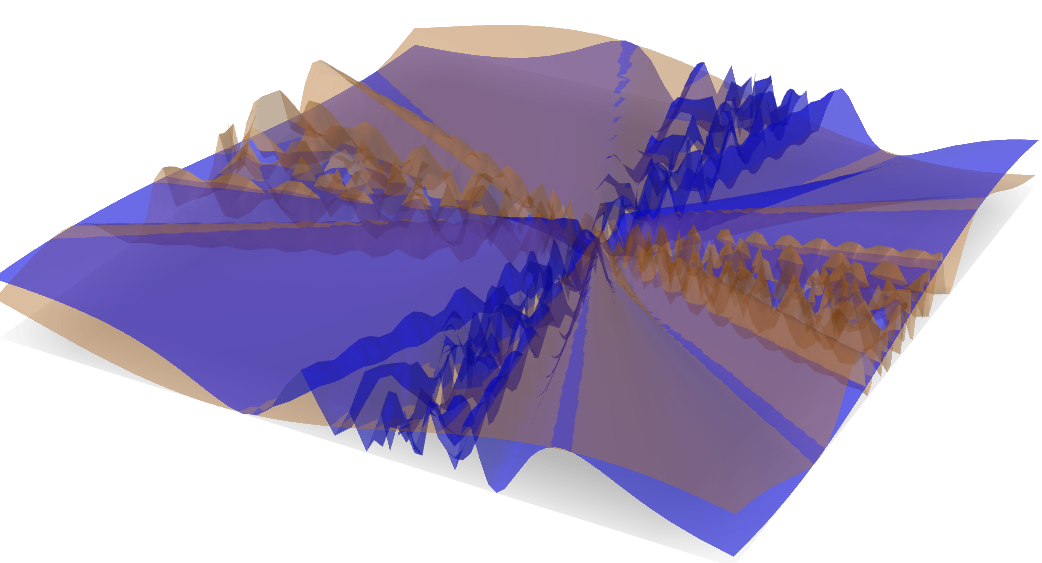
\includegraphics[scale=0.5]{C.png}

\begin{small}
The main purpose of these notes is to briefly remind the contents of it to those who already learnt them and to make a collection of the multivariable calculus subjects without going into too much detail.
\end{small}
\newpage
\tableofcontents
\newpage
\section{Analytic Geometry and Vectors in 3-Space}
Vectors are quantities that involve both magnitude and direction. They are shown by $\overrightarrow{AB}$ or \textbf{AB}.

Unit Vectors: $$\hat{v}=\frac{\vec v}{|\vec v|}$$
\subsection{Vector Operations}
\begin{enumerate}
\item Addition: $\overrightarrow{a} + \overrightarrow{b} = (a_1,a_2,a_3)+(b_1,b_2,b_3)=(a_1+b_1,a_2+b_2,a_3+b_3) $.
\item Scalar Multiplication: $c\cdot \overrightarrow{a}=c\cdot (a_1,a_2,a_3)=(c\cdot a_1, c\cdot a_2, c\cdot a_3)$ where $c\in \mathbb{R}$.
\item Dot Product: $\vec{a} \dotp \vec b  = (a_1,a_2,a_3)\dotp (b_1,b_2,b_3)= a_1 b_1+a_2 b_2+ a_3 b_3$. 

Geometric property of dot product is that it gives the \textbf{magnitude of projection of one operand vector to the other}. 

$\vec{a} \dotp \vec{b}= |\vec{a}||\vec{b}|\cos \theta$ where $\theta$ is the angle between $\vec a$ and $\vec b$ and $  (0 \leq \theta \leq \pi)$.

Scalar Projection of $\vec u $ in the direction of $\vec v \neq \vec 0$ is $$s= \vec u \dotp \hat v .$$

Vector Projection of $\vec u $ in the direction of $\vec v \neq \vec 0$ is $$\vec P = (\vec u \dotp \hat v) \hat v = \frac{\vec u \dotp \vec v}{|v|^2} v .$$
\item Cross Product: Where $\vec a= (a_1,a_2,a_3)$ and $\vec b=(b_1,b_2,b_3)$,\\ $\vec a \times \vec b = (a_2b_3-a_3b_2)\hat i + (a_3b_1-a_1b_3)\hat j+ (a_1b_2-a_2b_1)\hat k$

Cross Product results in a vector of the \textbf{magnitude of the area of the parallelogram created by the operand vectors} since $\vec a \times \vec b = |\vec a||\vec b|\sin \theta$ where $\theta$ is the angle between \textbf{a} and \textbf{b} vectors and that vector is \textbf{perpendicular to both operands}.

Lagrange's Identity: $$ |\vec a \times \vec b |^2= |\vec a|^2|\vec b|^2 - (\vec a \dotp \vec b)^2$$
Cab-bac formula: $$\vec a \times (\vec b \times \vec c) = (\vec c \dotp \vec a)\vec b - (\vec b \dotp \vec a)\vec c$$
\item Mixed Product: $$\vec a \dotp (\vec b \times \vec c)$$
Mixed Product operation gives the volume of the parallelepiped made up by vectors \textbf{a}, \textbf{b} and \textbf{c}.
\end{enumerate}
\subsection{Lines}
$$L: (x,y,z) = (x_0,y_0,z_0) + \lambda (p,q,r)$$
We use \textbf{parametric} equation and \textbf{symmetric (standard)} equation notations for lines in $\mathbb{R}^3$
\begin{equation}
	\tag{Parametric}
	x=x_0+\lambda p \ ,\  y=y_0 + \lambda q \ ,\  z=z_0+\lambda r
\end{equation}
\begin{equation}
	\tag{Standard}
	\frac{x-x_0}{p}=\frac{y-y_0}{q}=\frac{z-z_0}{r}= \lambda
\end{equation}
It must be noted that we only need \textbf{a point and a direction vector} or \textbf{two points in} order to obtain a \textbf{unique line equation}.

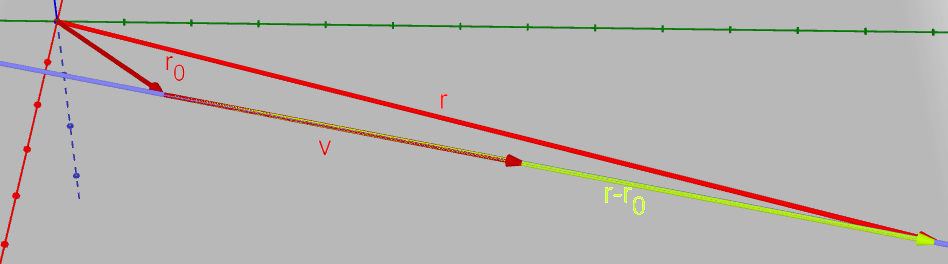
\includegraphics[scale=0.55]{line.png}

Equation is derived from the fact $\vec v \times (\vec r - \vec r_0)$.
\subsection{Planes}
$$Ax+By+Cz+D=0$$ is the equation for a plane that passes through $(x,y,z)=\left( -\frac{D}{3A},-\frac{D}{3B},-\frac{D}{3C}\right)$ and has normal vector $\vec n =(A,B,C)$. As understood, \textbf{a normal vector and a point on the plane, a line and a point outside of the line or three non-linear} points are sufficient to create a plane. However, a line only or just two points end up creating infinite number of planes.

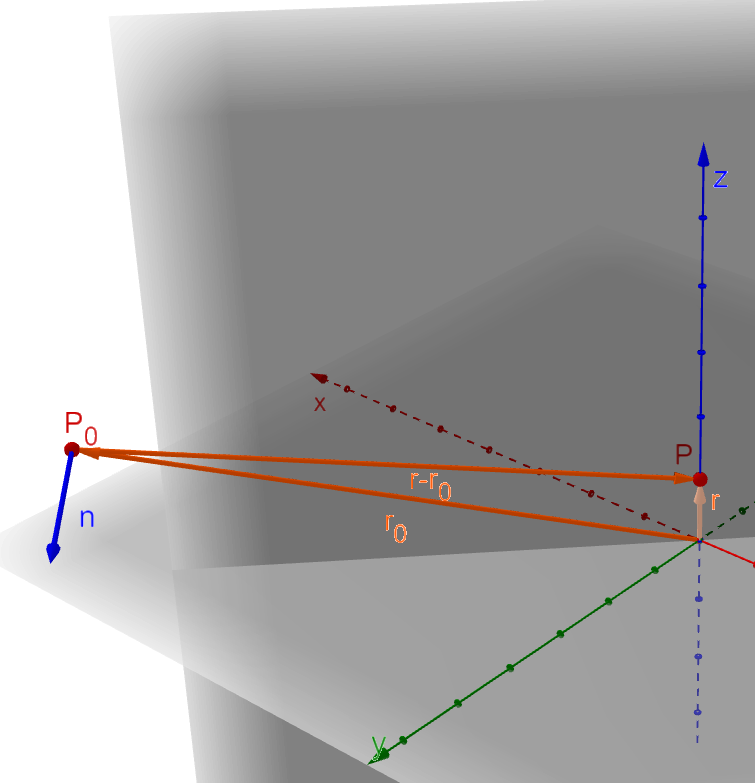
\includegraphics[scale=0.7]{plane.png}

Equation is derived from the fact $\vec n \dotp (\vec r - \vec r_0)=0$.
\newpage
\subsection{Distance Formulas}
\subsubsection{Point-Point Distance}
Let $ A =(x_0,y_0,z_0)$ and $B= (x_1,y_1,z_1)$. Then the distance between points A and B, $$|AB|= \sqrt{(x_1-x_0)^2+(y_1-y_0)^2+(z_1-z_0)^2}$$
\subsubsection{Point-Line Distance}
Let $L: (x,y,z) = (x_0,y_0,z_0) + \lambda (p,q,r)$ , $\vec d = (p,q,r)$, $\vec A=(x_0,y_0,z_0)$ (in fact, A can be any arbitrary point on the line L) and $\vec B=(x_1,y_1,z_1)$. Then distance between point $B$ and line $L$ is $$|(\vec B - \vec A)\times \hat d\,|.$$

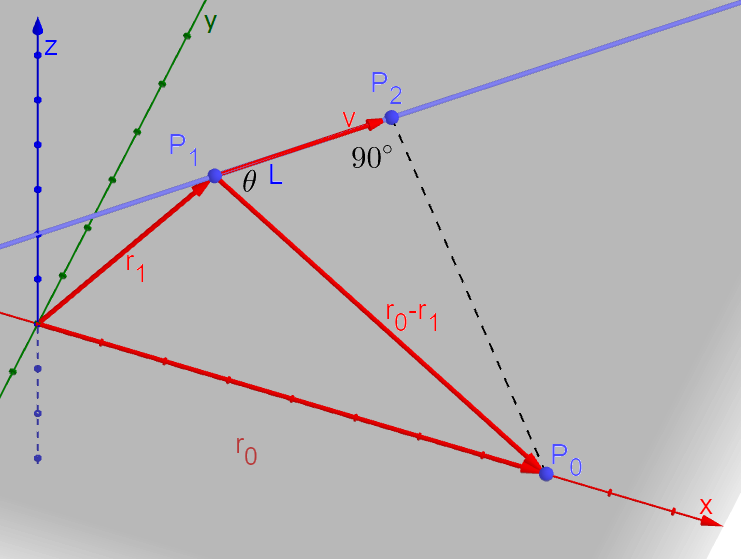
\includegraphics[scale=0.715]{pln.png}

\newpage
\subsubsection{Line-Line Distance}
In 3 dimensional systems, lines can have three relative positions, one being the lines \textbf{intersecting}, other being the lines being \textbf{parallel} to each other and the last is the lines being \textbf{skew} lines which means that the lines \textbf{neither intersect nor are they parallel} to each other. For the distance between them:

Let $L$ and $N$ be lines on 3-space and let $L$ pass through point $A$ and have directional vector $d_1$ and respectively, let $N$ pass through point $B$ and have directional vector $d_2$. Then distance between those lines is
$\displaystyle{\frac{|(\vec B - \vec A)\dotp(\vec d_1 \times \vec d_2)|}{|\vec d_1 \times \vec d_2|}}$ and if $(\vec d_1 \times \vec d_2 = \vec 0)$, then the lines are parallel and the distance between them is given by $\displaystyle{\frac{|(\vec B - \vec A)\times \vec d_1|}{|\vec d_1|}}$.

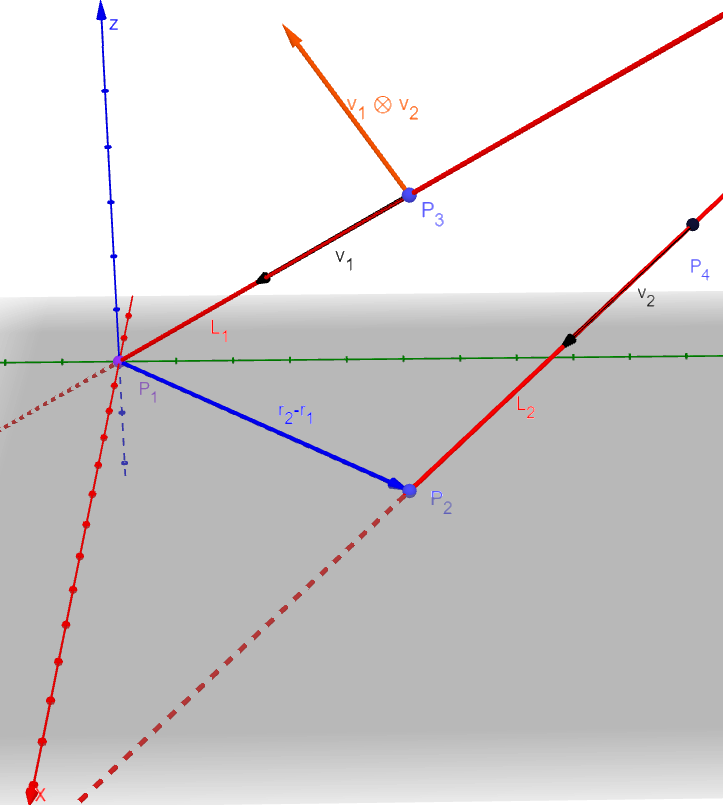
\includegraphics[scale=0.65]{lnln.png}

\newpage
\subsubsection{Line-Plane Distance}
The only possible way that a line and a plane having a distance different than 0 is that the \textbf{line's direction vector and plane's normal vector are perpendicular}, so:

Let $A$ be a point on line $L$ which has the direction vector $\vec d$ and let $B$ a point on the plane $P$ that has $\vec n$ normal vector. Then the distance between that line and plane would be $\displaystyle{\left|\vec{AB} \dotp \hat n\right|}$ where $\vec n \dotp \vec d =0$ and if $\vec n \dotp \vec d \neq 0$, distance between the vectors would be 0.
\subsubsection{Point-Plane Distance}
Let $K$ be a point anywhere on $\mathbb{R}^3$ and let plane $P: Ax+By+Cz-D=0$ which has the normal vector $\vec n = (A,B,C)$ and passes through an arbitrary point $M$. Then the distance from point $K$ to the plane is $$|\vec{MK}\dotp \hat n|$$ or $$\dfrac{|Ax_K+By_K+Cz_K-D|}{\sqrt{A^2+B^2+C^2}}$$
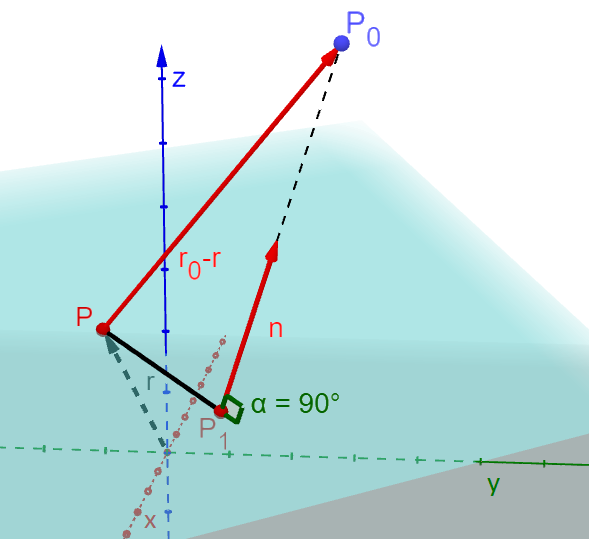
\includegraphics[scale=0.7]{pointplane.png}

\subsubsection{Plane-Plane Distance}
If and only if the planes are parallel, they could have a distance different than zero. 

Let $P_1$ and $P_2$ be planes on 3-space which have the mutual normal vector $\vec n$ and let point $A$ be on plane $P_1$ and point $B$ be on plane $P_2$. Then the distance of the planes will be $$|\vec{AB} \dotp \hat n|$$
\section{Vector-Valued Functions}
Vector-valued functions, if defined on $\mathbb{R}^3$ and graphed under 3-space, indicate a curve in space, such as the orbit of a particle and as such, the derivatives of such functions give the tangential vector, we could call velocity of the particle. In physics, generally the parameter of such functions is time but in mathematics, it must be noted that it is just a parameter, not necessarily intuitive.
\subsection{Parametrizations}
We can find the curves of intersection of two surfaces and with vector-valued functions, express them. It is important to know that such curves can be parametrized in many, possibly infinite ways. However, some parametrizations of a curve can prove to be much easier where the others are relatively cumbersome. 
\subsection{Arc-length}
Let $\vec r(t)$ be a vector-valued function and let $\vec v(t)=\dfrac{d\vec r}{dt}$. Then the arc length L:
$$L= \int \limits_a^b |\vec v(t) | dt.$$
\newpage
\section{Multivariable Functions}
\subsection{Defining Multivariable Functions}
Let $\mathbb{D}\in\mathbb{R}^2$, a rule $f$ which assigns every point of $\mathbb{D}$ a unique real number is called a function of two variables.
\subsection{Quadric Surfaces}
Equations of form $Ax^2+By^2+Cz^2+Dxy+Exz+Fyz+Gx+Hy+Iz+K=0$ where at least one second degree term is nonzero. 

To draw, the most reliable method is to first see intersection with coordinate planes and if required, other arbitrary planes. 

Some important quadric surfaces:
\begin{enumerate}
\item \textbf{Elliptic Cone}: $$z^2=\frac{x^2}{a^2}+\frac{y^2}{b^2}$$ where $a,b\in \mathbb{R}$.

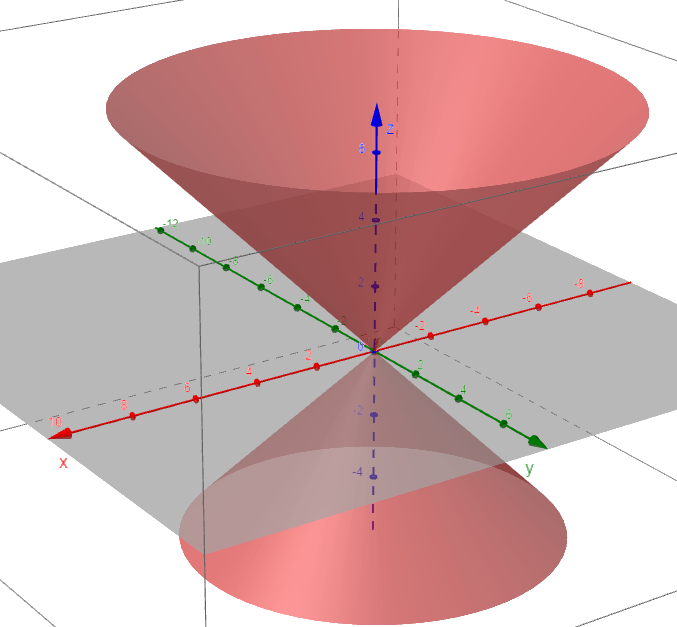
\includegraphics[scale=0.70]{cone.png}

\item \textbf{Elliptic Paraboloid}: $$z=\frac{x^2}{a^2}+\frac{y^2}{b^2}$$ where $a,b\in \mathbb{R}$.

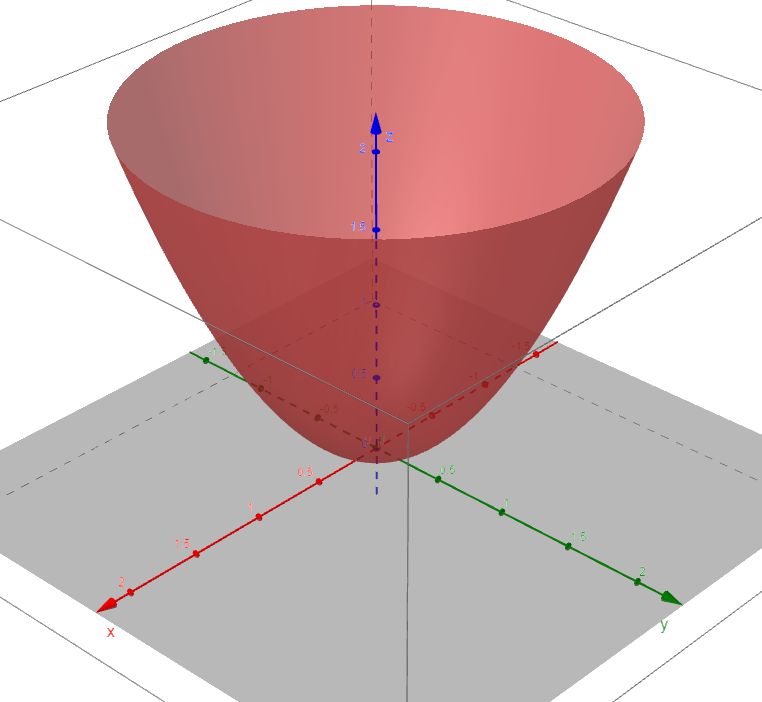
\includegraphics[scale=0.65]{paraboloid.png}

\newpage
\item \textbf{Hyperboloid of one sheet}: $$\frac{x^2}{a^2}+\frac{y^2}{b^2}-\frac{z^2}{c^2}=1$$ where $a,b,c \in \mathbb{R}$.

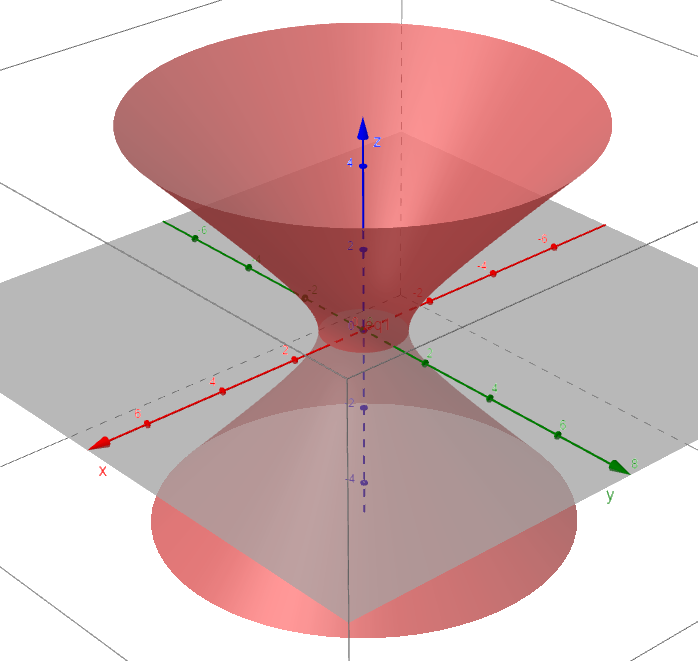
\includegraphics[scale=0.74]{hy_1.png}

\newpage
\item \textbf{Hyperboloid of two sheets}: $$\frac{x^2}{a^2}+\frac{y^2}{b^2}-\frac{z^2}{c^2}=-1$$ where $a,b,c \in \mathbb{R}$.

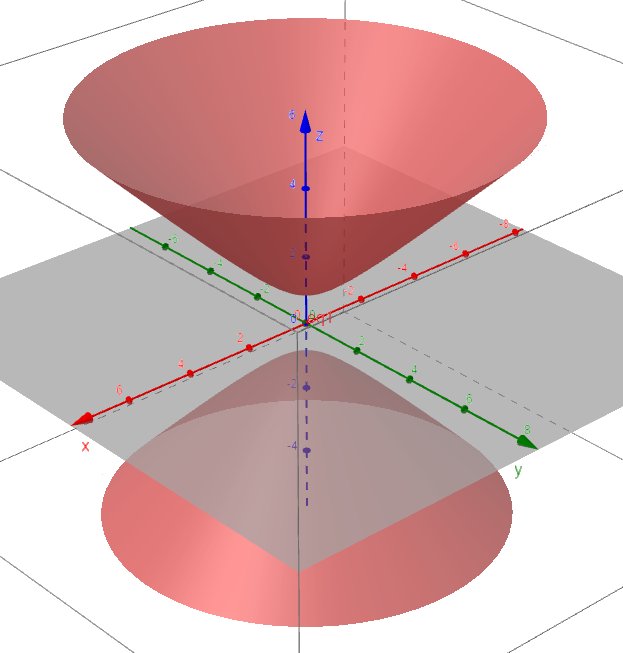
\includegraphics[scale=0.75]{hy_2.png}

\item \textbf{Ellipsoid}: $$\frac{x^2}{a^2}+\frac{y^2}{b^2}+\frac{z^2}{c^2}=1$$ where $a,b,c \in \mathbb{R}$.

\newpage
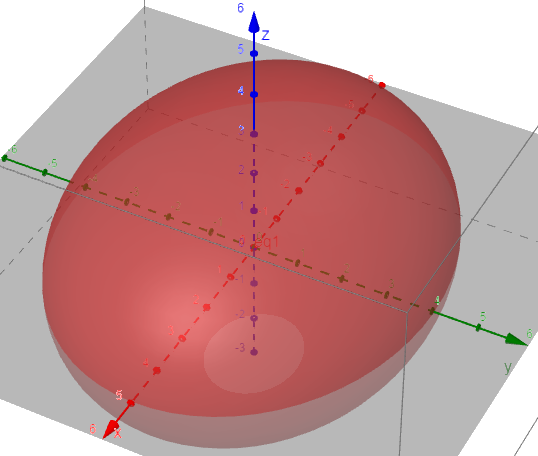
\includegraphics[scale=0.7]{ellipsoid.png}

\item \textbf{Hyperbolic Paraboloid (Saddle Surface)}: $$z=\frac{y^2}{b^2}-\frac{x^2}{a^2}$$ where $a,b\in \mathbb{R}$

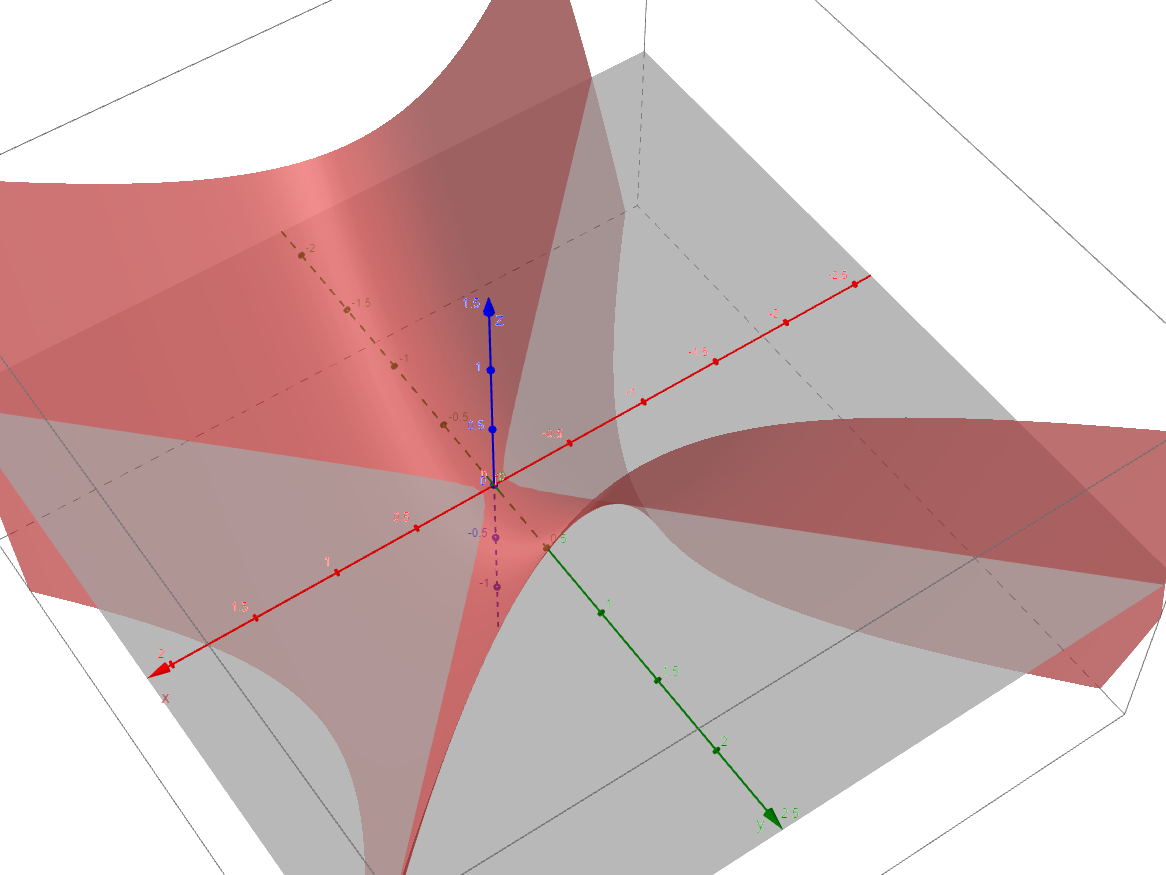
\includegraphics[scale=0.4]{saddle.png}

\item \textbf{Sphere}: $$x^2+y^2+z^2=r^2$$ where $r\in \mathbb{R}$.

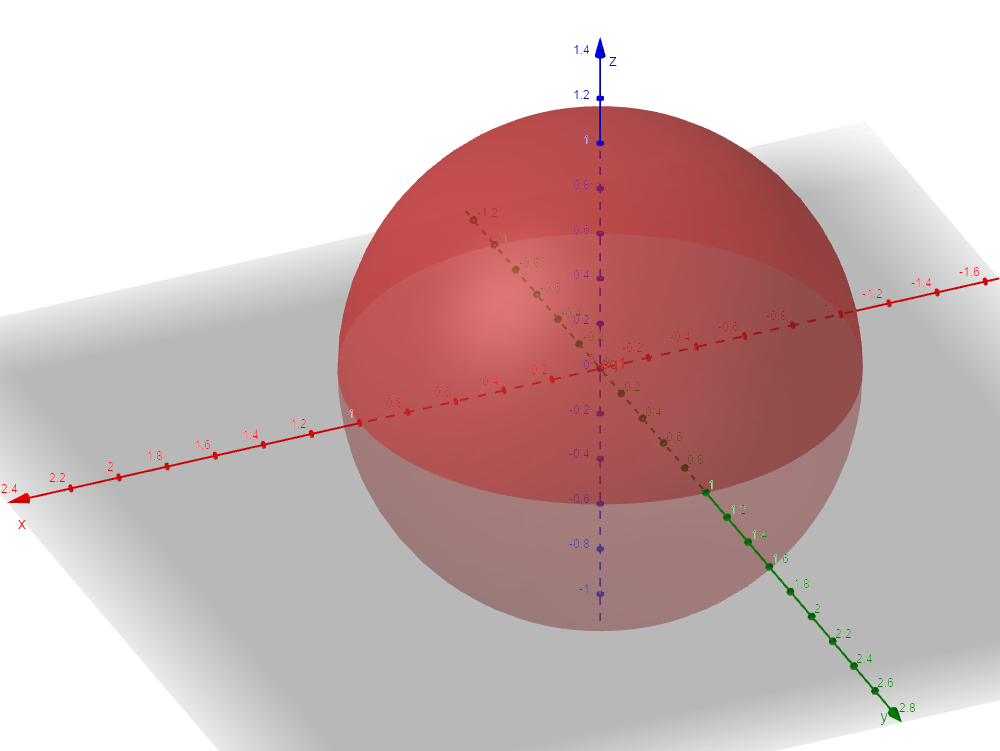
\includegraphics[scale=0.5]{sphere.png}

\end{enumerate}
\subsection{Cylinders}
A cylindrical surface is a surface consisting of all the points on all the lines which are parallel to a given line and which pass through a fixed plane curve in a plane not parallel to the given line.

A solid bounded by a cylindrical surface and two parallel planes is called a (solid) cylinder.

Cylinders can be oblique or right cylinders. Right cylinders appear when the \textbf{equation of the surface does not contain one of the 3-space variables}.
\newpage
\subsection{Level Curves}
Let $f$ be a function of two variables. The curve $f(x,y)=c$ is called a level curve when $c\in\mathbb{R}$. Level curves are used to build topographic maps and contour plots of surfaces. 

\begin{figure}[H]
\centering
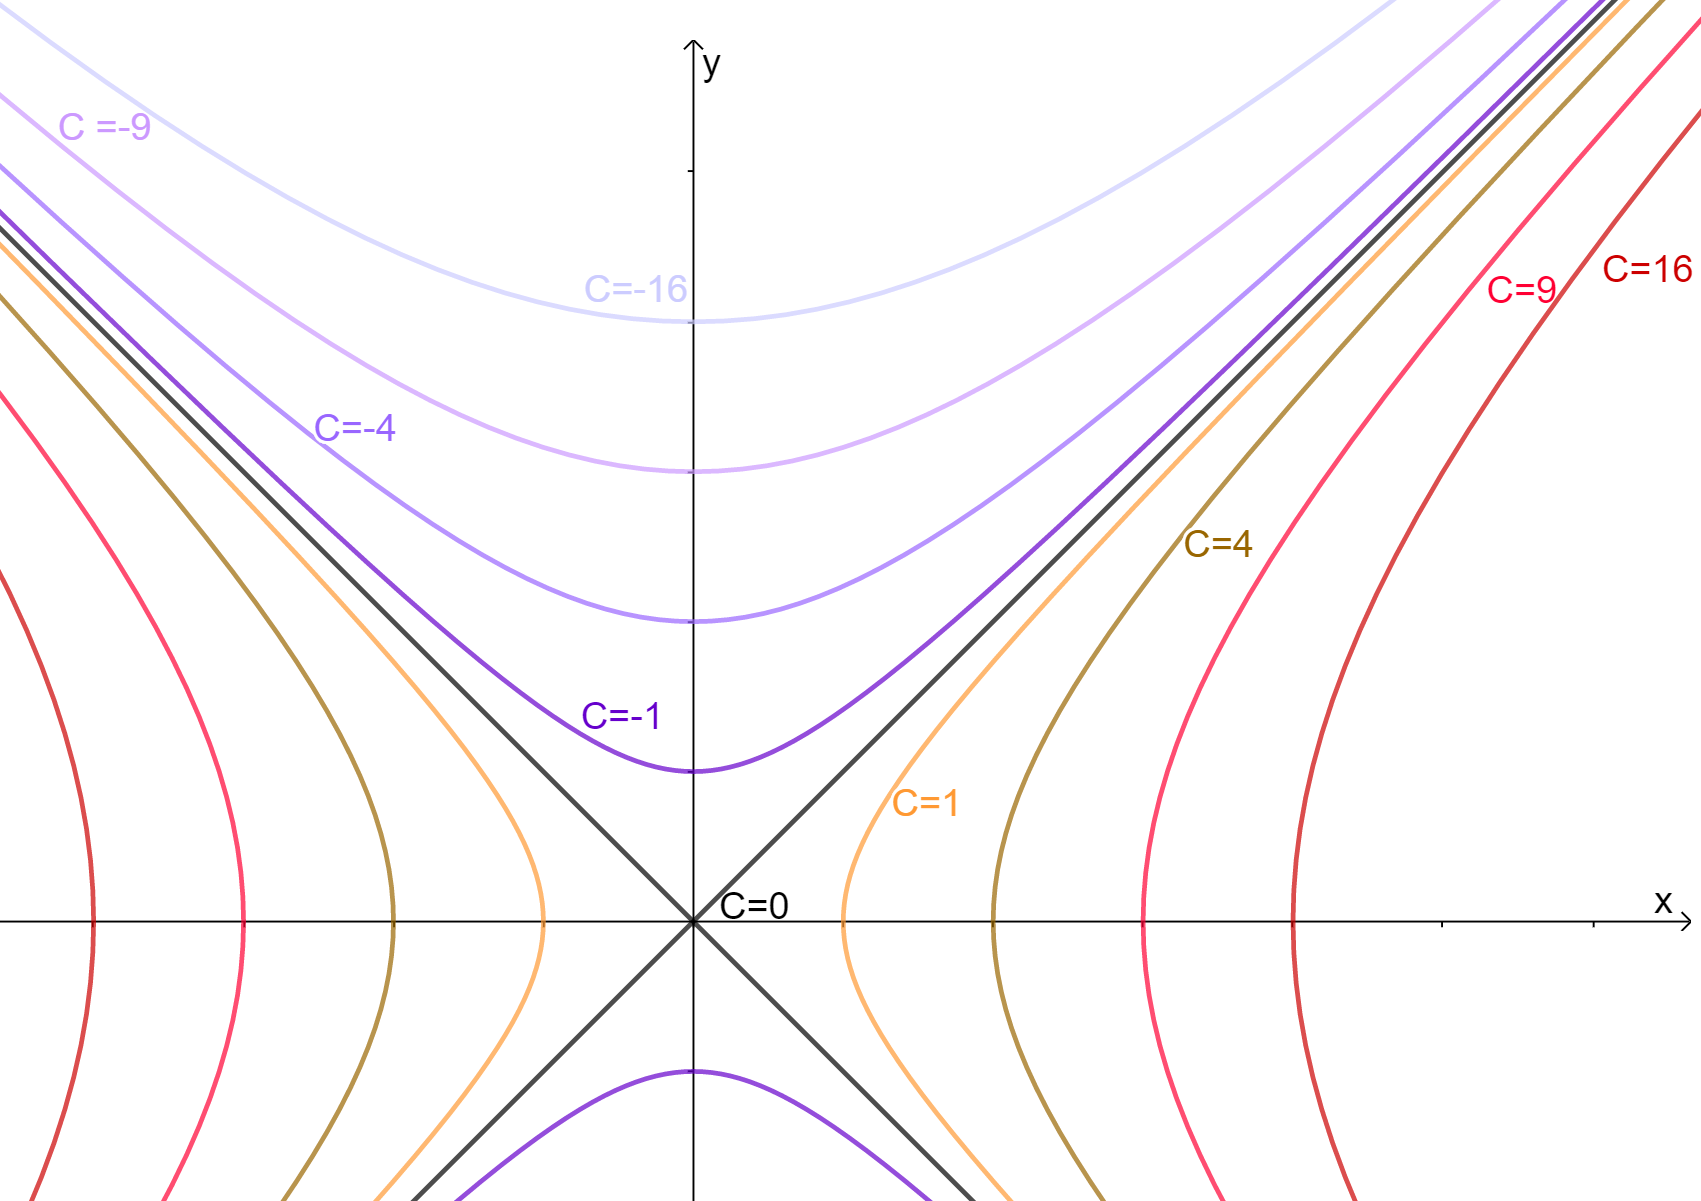
\includegraphics[scale=0.3]{levelcurve.png}
\caption{Level curves of a saddle surface}
\end{figure}

\newpage
\subsection{Level Surfaces}
Let $f$ be a function of three variables. The surface $f(x,y,z)=c$ is called a level surface when $c\in\mathbb{R}$. Since we can not visualize functions with three -or more- variables as graphs, the closest we could visually operate on them is to use level surfaces.


\begin{figure}[H]
\centering
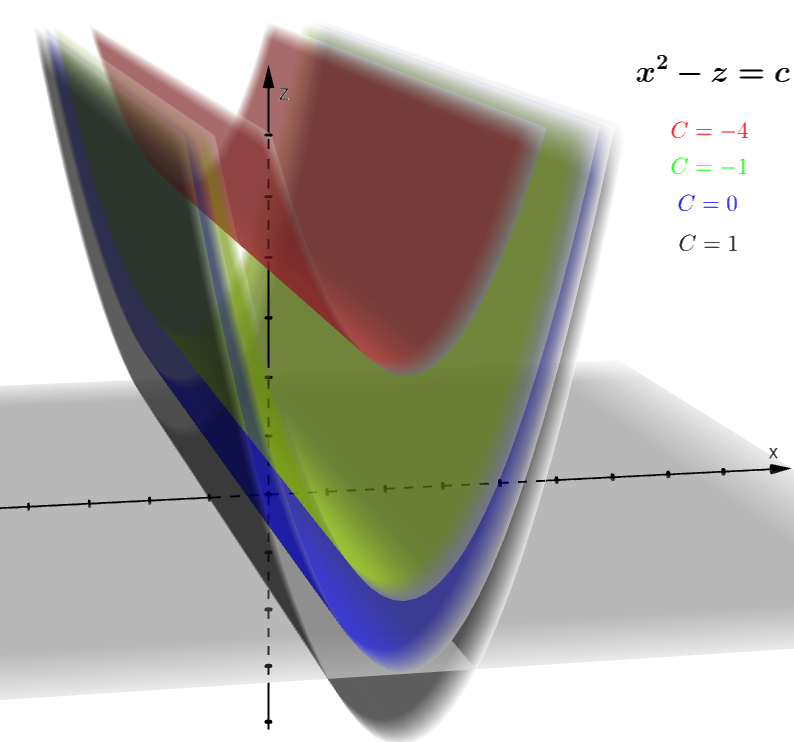
\includegraphics[scale=0.66]{levelsurf.png}
\caption{Level surfaces of $f(x,y,z)=x^2-z$}
\end{figure}

\newpage
\subsection{Polar Coordinates}
While rectangular coordinates are shown on $x$ and $y$ axis, the polar coordinates are shown as $\theta$ and $r$ where $\theta$ is the angle made with $x$ axis and $r$ is the distance away from the origin. In this sense $$x=r \cos \theta \ ,\ y=r \sin \theta \ ,\ r=\sqrt{x^2+y^2} \ , \ \theta = \arctan |\frac{y}{x}| \ldots(x\neq 0).$$
However the transformations are not necessarily unique since: 
$$(r,\theta)=(-r,\theta +\pi)= (r,\theta +2\pi )$$
Hence it is useful to define $0 \leq \theta \leq 2\pi$ and develop two representations where $r$ can only be non-negative ($+r$ representation) or $r$ can be only non-positive ($-r$ representation).
\subsubsection{Polar Curves}
\begin{enumerate}
\item \textbf{Line}: To represent a line that passes from the origin and has slope angle, $\phi$ $$\theta=\phi$$
\item \textbf{Circle}: To represent a circle centered around origin with radius $R$, $$r=R$$
\newpage
\item \textbf{Limaçons}: $$r = b \pm a \cos \theta \ \vee r= b \pm a \sin \theta$$
If $\frac{b}{a}<1$, limaçon appears with an inner loop.

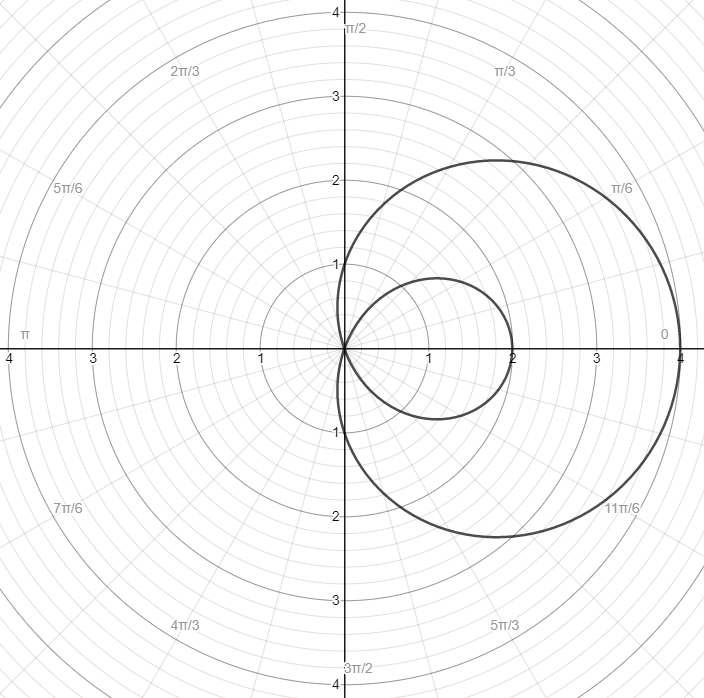
\includegraphics[scale=0.7]{innerloop.png}

\newpage
If $1 < \frac{b}{a}<2$, limaçon appears with a dimple.

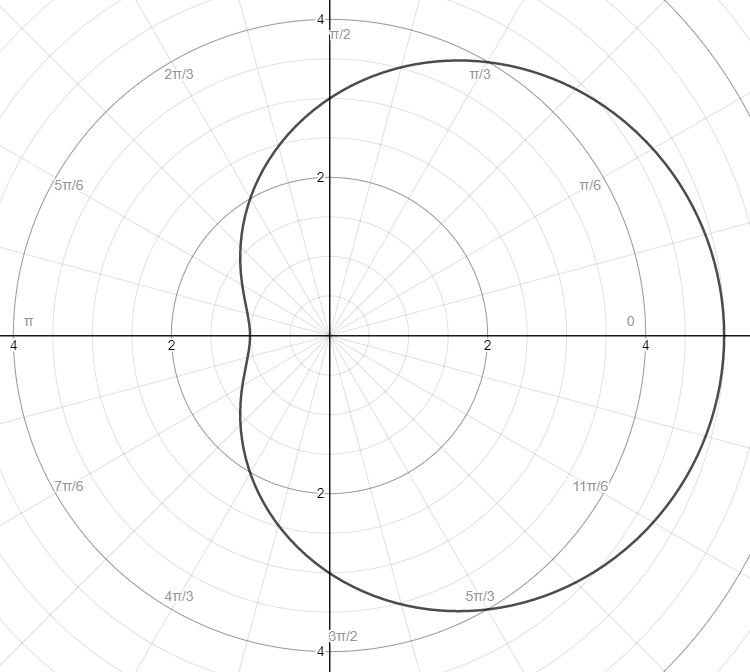
\includegraphics[scale=0.688]{dimple.png}

\newpage
If $\frac{b}{a} \geq 2$, limaçon is convex.

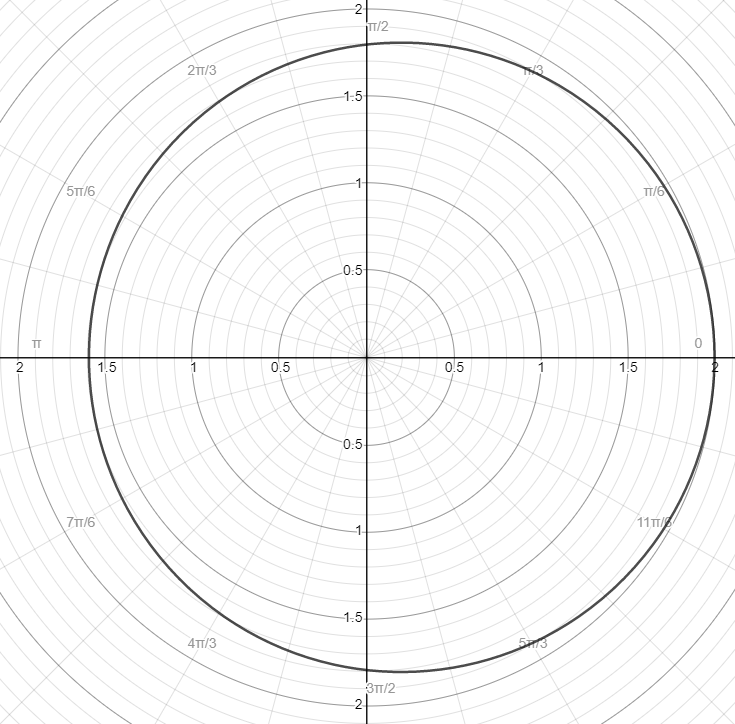
\includegraphics[scale=0.7]{convex_lim.png}

\newpage
\item \textbf{Cardioid}: Limaçons in which $a=b$, $$r=a(1 \pm \cos \theta) \vee r=a(1 \pm \sin \theta)$$

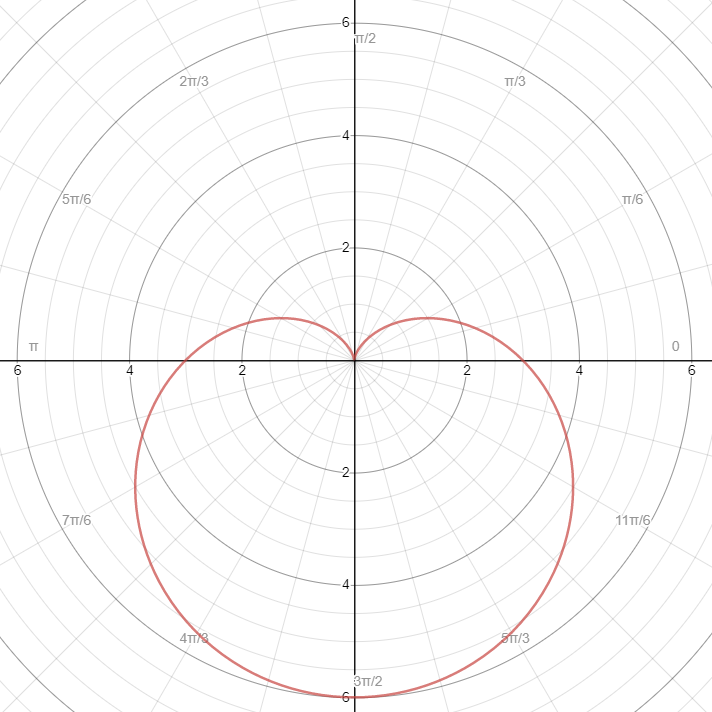
\includegraphics[scale=0.5]{cardioid.png}

\newpage
\item \textbf{Rose Curves}: $$r= a \cos n\theta \vee r=a \sin n\theta$$
If $n$ is odd, the rose has $n$ petals and if $n$ is even, the rose has $2n$ petals. As seen, we can not have a rose curve with two petals with this formulation.
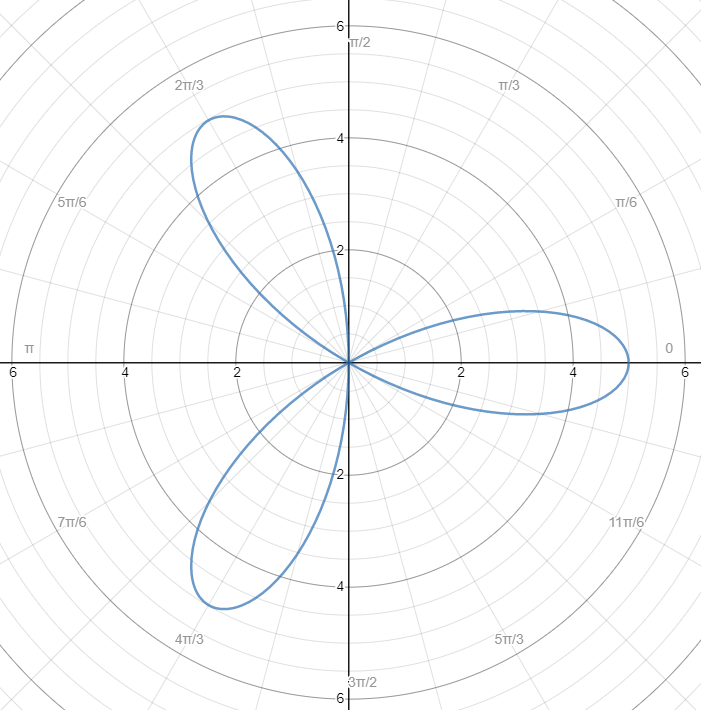
\includegraphics[scale=0.6]{rose.png}

\newpage
\item \textbf{Lemniscates}: Two loops (petals), $$r^2=a^2 \cos 2\theta \vee r^2= a^2 \sin 2\theta$$
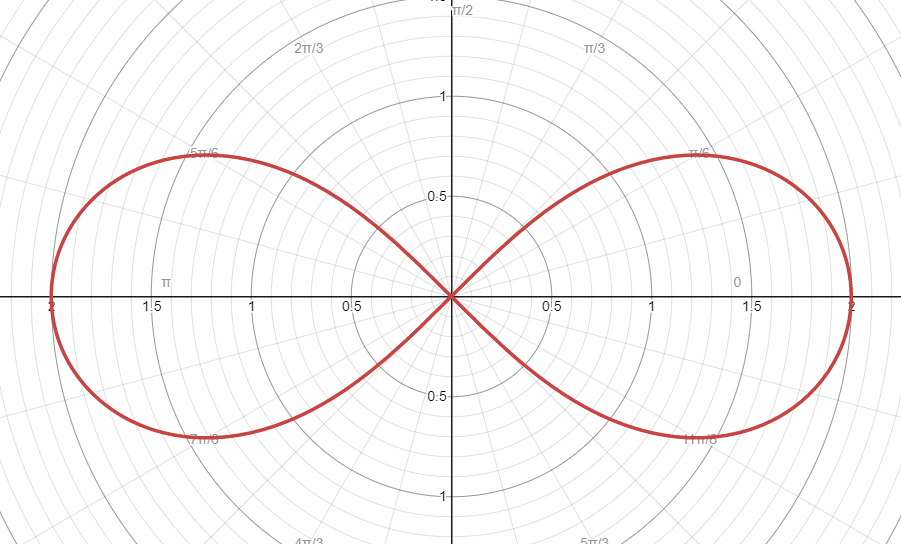
\includegraphics[scale=0.57]{lemniscate.png}

\end{enumerate}
\subsubsection{Drawing Polar Curves}
\begin{enumerate}
\item \textbf{Symmetry}: Symmetry in polar curves can help us narrow down the interval we check values with. If we have symmetry about y-axis, then we only need to draw accurately, the function on $-\frac{\pi}{2}\leq \theta \leq \frac{\pi}{2}$ and if we have symmetry about x-axis, we only have to draw $0 \leq \theta \leq \pi$ and if there is symmetry about the origin, we only need to draw two adjacent quadrants.

If $f(-\theta)=f(\theta)$ ,then the function shows \textbf{symmetry about x-axis}.

If $f(\pi - \theta)=f(\theta)$, then the function shows \textbf{symmetry about y-axis}. 

If $f(\theta +\pi)=f(\theta)$, then the function shows \textbf{symmetry about the origin}.
\item \textbf{Consider General Formulations}: If the given function that need to be drawn is already memorized, then it is easier to draw it directly or to use the memorized curve's properties about symmetry and shape-wise details as clues regarding the drawing of the curve.
\item \textbf{Check points}: Try as much as relatively easily calculable angle values within the interval that has been determined by the symmetry of the given curve.

\end{enumerate}
\subsubsection{Intersection of Polar Curves}
Since the transformations between rectangular and polar coordinates are not necessarily unique, finding intersections of two curves can be difficult. One way is to find all solutions to the system of equations for the intersecting systems and then drawing the graph for the other possibly existent intersections. One other way that was not given on the class texts is to regard given curves as two different curves such that one curve $r(\theta) \Rightarrow -r(\theta +\pi)$ and actually solve 4 systems of equations (solving 2 of them is enough but sometimes knowing which two of the possible 4 might be difficult). 
\subsubsection{Cylindrical Coordinates}
$$x=r \cos \theta \ ,\ y= r \sin \theta \ ,\ z=z.$$
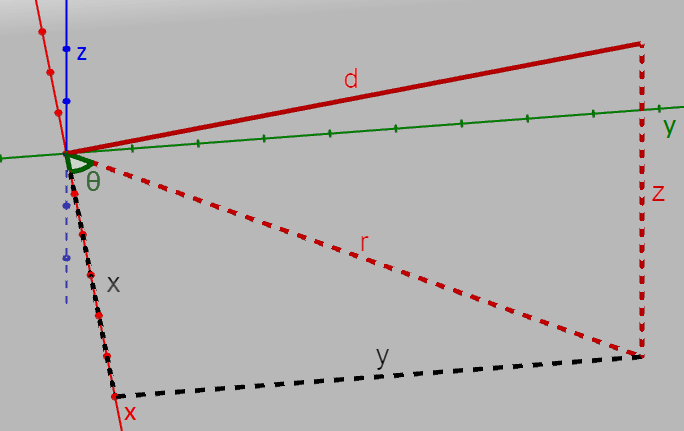
\includegraphics[scale=0.8]{cylindr_co.png}

\newpage
\subsubsection{Spherical Coordinates}
$$x=R\sin \phi \cos \theta \ , \ y=R \sin \phi \sin \theta \ , \ z=R \cos \theta$$
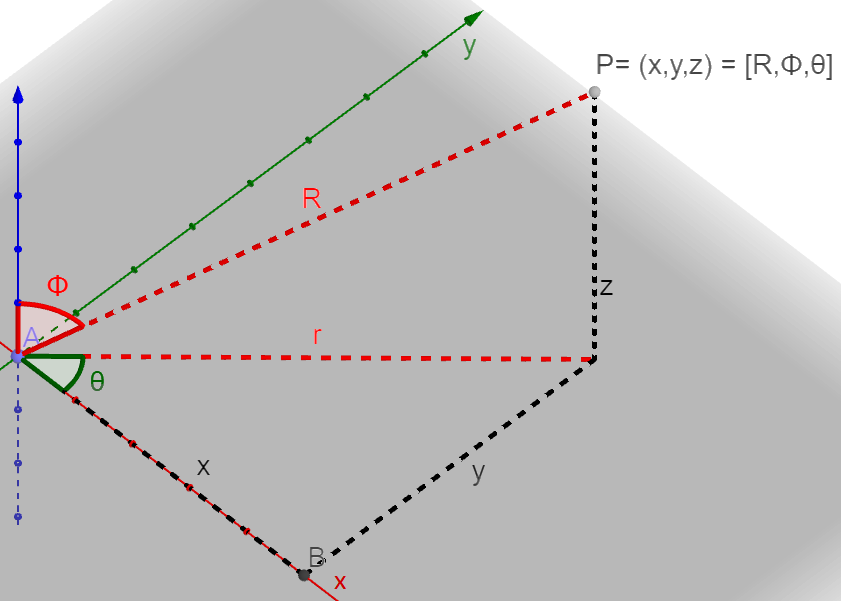
\includegraphics[scale=0.65]{spherical_co.png}

\newpage
\section{Limits and Continuity}
We used to consider limits approaching from the two sides for functions of one variable. Here we can not see two sides of a limit, rather, there is a disk shaped area which we can approach from, which means \textbf{there are infinite ways to approach to a limit of two -or more- variables}.
\subsection{Definition of Limit on Multivariable Functions}
Formal definition of limits for functions of two variables and the foundation of the formal definition of limits' for any amount of variables are the same and the following expression can be expanded for any amount of variables: 
$$\lim \limits_{(x,y)\to (a,b)}=L \Leftrightarrow (\forall \epsilon > 0) \Rightarrow (\exists \delta>0) :$$$$ \sqrt{(x-a)^2+(y-b)^2}<\delta\Rightarrow |f(x,y)-L|<\epsilon$$
\subsection{Taking Limits}
In limits of more than one variable, the only way to formally prove that the limit exists is using the \textbf{formal definition of limits} or if it can be used, usage of the \textbf{squeeze theorem}. Remember that we used to approach from both sides of a single variable limit in order to prove its existence and also its value, here, however we need to approach from infinite amount of directions in order to prove its existence which is impossible. The only way to use the approaching from different sides method is when it is believed that the limit does not exist and we can \textbf{prove the limit's nonexistence by approaching from different sides}:

Along path $P_1(x): \lim \limits_{(x,y) \to (x_0,y_0)}f(x,y)=L_1$

Along path $P_2(x):\lim \limits_{(x,y) \to (x_0,y_0)}f(x,y)=L_2$

And $L_1\neq L_2$ proves that the limit does not exist but again, this can not be used to show that a limit exists.
\subsection{Continuity}
Much like continuity of a single variable function, $f(x_0,y_0)$ is continuous if $$\lim \limits_{(x,y)\to (x_0,y_0)}f(x,y)=f(x_0,y_0).$$ If a function is continuous at each point of the domain $D$, then it is said to be continuous on D.
\section{Partial Differentiation}
\subsection{Newton Quotients for Partial Derivatives}
$$f_x(x,y)=\lim \limits_{h \to 0} \dfrac{f(x+h,y)-f(x,y)}{h}$$
$$f_y(x,y)=\lim \limits_{k \to 0} \dfrac{f(x,y+k)-f(x,y)}{k}$$
\subsection{Partial Derivative Notations}
$$\dfrac{\partial z}{\partial x} = \dfrac{\partial}{\partial x} f(x,y) = f_1(x,y)=f_x(x,y)=D_1f(x,y)$$
$$\dfrac{\partial^2 z}{\partial x^2} = \dfrac{\partial^2}{\partial x^2} f(x,y) = f_{11}(x,y)=f_{xx}(x,y)=D_{11}f(x,y)$$
$$\vdots$$
Note : $\displaystyle{f_{xy}(x,y)=f_{yx}(x,y)}$
\subsection{Differentiability}
$f(x,y)$ is differentiable at $(a,b)$ if $$\lim \limits_{(h,k)\to (0,0)} \dfrac{f(a+h,b+k)-f(a,b)-hf_x(a,b)-kf_y(a,b)}{\sqrt{h^2+k^2}}=0.$$

This is an ill-defined expression since it already assumes that $f_x$ and $f_y$ exists, however it is a good way to conclude the question "is $f(x,y)$ continuous at $(a,b)$?" after knowing that both $f_x$ and $f_y$ exists at the given point.
\subsection{Tangent Planes and Normal Lines}
Let $f(x,y)$ be a function of two variables which is differentiable at point $(a,b)$. Then the tangent plane equation is
$$P_T(x,y)= f_x(a,b)(x-a) + f_y(a,b)(y-b)+f(a,b)$$
which can be used to approximate near points. We see that this plane has the normal vector $\vec n = (f_x(a,b),f_y(a,b),-1)$ and as such a normal line can be generated as a line that passes through $(a,b,f(a,b))$ and that is parallel to $\vec n$. Then the line will have the standard form equation of $$\dfrac{x-a}{f_x(a,b)}=\dfrac{y-b}{f_y(a,b)} = \dfrac{z-f(a,b)}{-1}=\lambda.$$
\subsection{Gradient}
$$\nabla f(x,y)=f_x(x,y)\hat i + f_y(x,y) \hat j.$$
\begin{enumerate}
\item Given that the function $f(x,y)$ is differentiable at point $(a,b)$ and $\nabla f(a,b) \neq \vec 0$, $\nabla f(a,b)$ is a normal vector to the level curve of $f$ that passes through $(a,b)$.
\item $\nabla f(x,y) - \hat k$ is a normal vector to the surface of the function $f$.
\item $\nabla f(a,b,c)$ is normal vector to the level surface of function $f(x,y,z)$ which passes through $(a,b,c)$. 
\item Gradient vector points at the direction of the fastest increase at the taken point and gradient vector's magnitude is the maximum rate of increase, predictably, maximum rate of decrease is in the opposite direction of the gradient vector and the rate of decrease is still the gradient's magnitude.
\end{enumerate}
\subsubsection{Directional Derivatives}
Newton Quotient where $\hat u = n \,\hat i+ k \,\hat j$ :
$$D_{\hat{u}} f(a,b)= \lim \limits_{h \to 0} \dfrac{f(a+hn,b+hk)-f(a,b)}{h} .$$
Also: $$D_{\hat{u}} f(a,b) =\left. \dfrac{d}{dt} f(a+tn,b+tk) \right|_{t=0}$$
Using Gradients:
$$D_{\hat{u}} f(a,b) = \hat u \dotp \nabla f(a,b)$$
\subsection{Taylor Polynomials for Functions of Two Variables}
We have discussed the tangent planes and they are the first degree Taylor polynomials for a function of two variables. In fact, we can approximate functions with polynomials with any degree using Taylor expansions: 
$$f(x,y)= f(a,b)+f_x(a,b)(x-a)+f_y(a,b)(y-b)+$$$$\frac{f_{xx}(a,b)(x-a)^2}{2!}+\frac{f_{yy}(a,b)(y-b)^2}{2!}+2\cdot \frac{f_{xy}(a,b)(x-a)(y-b)}{2!} \hdots \ \ , [C=(a,b)]$$
Using the same logic, functions of more variables can be expressed as polynomials.
\subsection{Extrema}
Types of extrema:
\begin{enumerate}
\item A function is said to have an \textbf{absolute maximum} at $(x_0,y_0)$ if \\ $f(x_0,y_0)\geq f(x,y),\  \forall (x,y)\in D_f$.
\item A function is said to have an \textbf{absolute minimum} at $(x_0,y_0)$ if \\ $f(x_0,y_0)\leq f(x,y),\  \forall (x,y)\in D_f$.
\item $f(x_0,y_0)$ is a \textbf{relative maximum} if $f(x_0,y_0) \geq f(x,y),\  \forall (x,y)$ in an open disk containing $(x_0,y_0)$.
\item $f(x_0,y_0)$ is a \textbf{relative minimum} if $f(x_0,y_0) \leq f(x,y),\  \forall (x,y)$ in an open disk containing $(x_0,y_0)$.
\end{enumerate}
Conditions for extrema:
\begin{enumerate}
\item Extremum points are where $\nabla f = \vec 0$ (\textbf{critical points} of $f$),
\item Extremum points are where $\nabla f$ does not exist (\textbf{singular points} of $f$),
\item Extremum points are the \textbf{boundary points} of $D_f$. It is important to observe that if we are working with a restricted domain, the points on the restriction path also need to be checked for extremum conditions.
\end{enumerate}
\subsubsection{Classifying Critical Points}
There are three types of critical points: \textbf{maximum, minimum or saddle points}. We can not classify these points only using first derivatives and as such we have a \textbf{second derivative test} that is derived from the \textbf{second degree Taylor polynomials' discriminant} :
$$D = f_{xx}f_{yy}-f_{xy}^2$$
\begin{enumerate}
\item A \textbf{relative maximum} occurs at a critical point whose $D>0$ and $f_{xx}<0$ (or $f_{yy}<0$).
\item A \textbf{relative minimum} occurs at a critical point whose $D>0$ and $f_{xx}>0$ (or $f_{yy}>0$).
\item A \textbf{saddle point} is found at a critical point whose $D<0$.
\item If $D=0$, then the \textbf{test is inconclusive} and results from the higher degree Taylor polynomials must be investigate to conclude.

\end{enumerate}
\subsection{Lagrange Multipliers}
The method of Lagrange multipliers is used to solve the extreme values of functions subjected to other other functions. The method's key points are those that we are actually caring about the \textbf{level curves} of functions rather than the surfaces and we solve the optimization problem by the fact that these \textbf{level curves must be tangentially intersecting each other in the optimum scenario}. We can sum up by saying if there is a function $f(x,y)$ constrained with the curve $g(x,y)=c$, the optimum-value can be found using Lagrange multipliers by stating three equations:
\begin{align}
	\nabla f(x,y) \dotp \hat i &=\lambda \nabla g(x,y) \dotp \hat i \\
	\nabla f(x,y) \dotp \hat j &=\lambda \nabla g(x,y) \dotp \hat j \\
	g(x,y)&=c
\end{align}

Such problem is formed with functions of two variables above however this method is applicable to functions with any number of variables, as long as they form a solvable system, for example when $\nabla g =0$ the method can not operate, or if the optimum point lies on the endpoint of the $g(x,y)=0$ curve. Moreso, the method can be applied with more than one constraint, if in addition to the above formulation, $h(x,y)=k$
\begin{align}
	\nabla f(x,y) \dotp \hat i &=\lambda \nabla g(x,y) \dotp \hat i + \mu \nabla h(x,y) \dotp \hat i \\
	\nabla f(x,y) \dotp \hat i &=\lambda \nabla g(x,y) \dotp \hat i + \mu \nabla h(x,y) \dotp \hat i \\
	g(x,y)&=c\\
	h(x,y)&=k
\end{align}

In conclusion, as with all equation solving, if the amount of independent equations are equal to the amount of independent variables, the equation can be solved and as such systems with any number of variables and any number of constraints can be generated and solved with Lagrange's method.
\newpage
\section{Multiple Integration}
\subsection{Fubini's Theorem}
$$\iint \limits_{X\  Y} f(x,y)\,dA=\int \limits_X \int \limits_Y f(x,y)\,dy\,dx=\int \limits_Y \int \limits_X f(x,y)\,dx\,dy$$
$$\iiint \limits_{XYZ} f(x,y,z)\, dV=\int \limits_X \int \limits_Y \int \limits_Z f(x,y,z)\,dz\,dy\,dx =\int \limits_Z \int \limits_Y \int \limits_X f(x,y,z)\,dx\,dy\,dz \cdots$$
Fubini's theorem simply states that \textbf{multiple integrals can be expanded into iterated integrals}. Then, iterated integration can theoretically be performed in \textbf{any order} as long as we \textbf{adjust the integral boundaries carefully} however sometimes one order can lead to non-elementary functions or unsolvable integrals even, in those cases the order must be reconsidered.
\subsection{Double Integrals}
\subsubsection{Double Integrals Over a Rectangular Area}
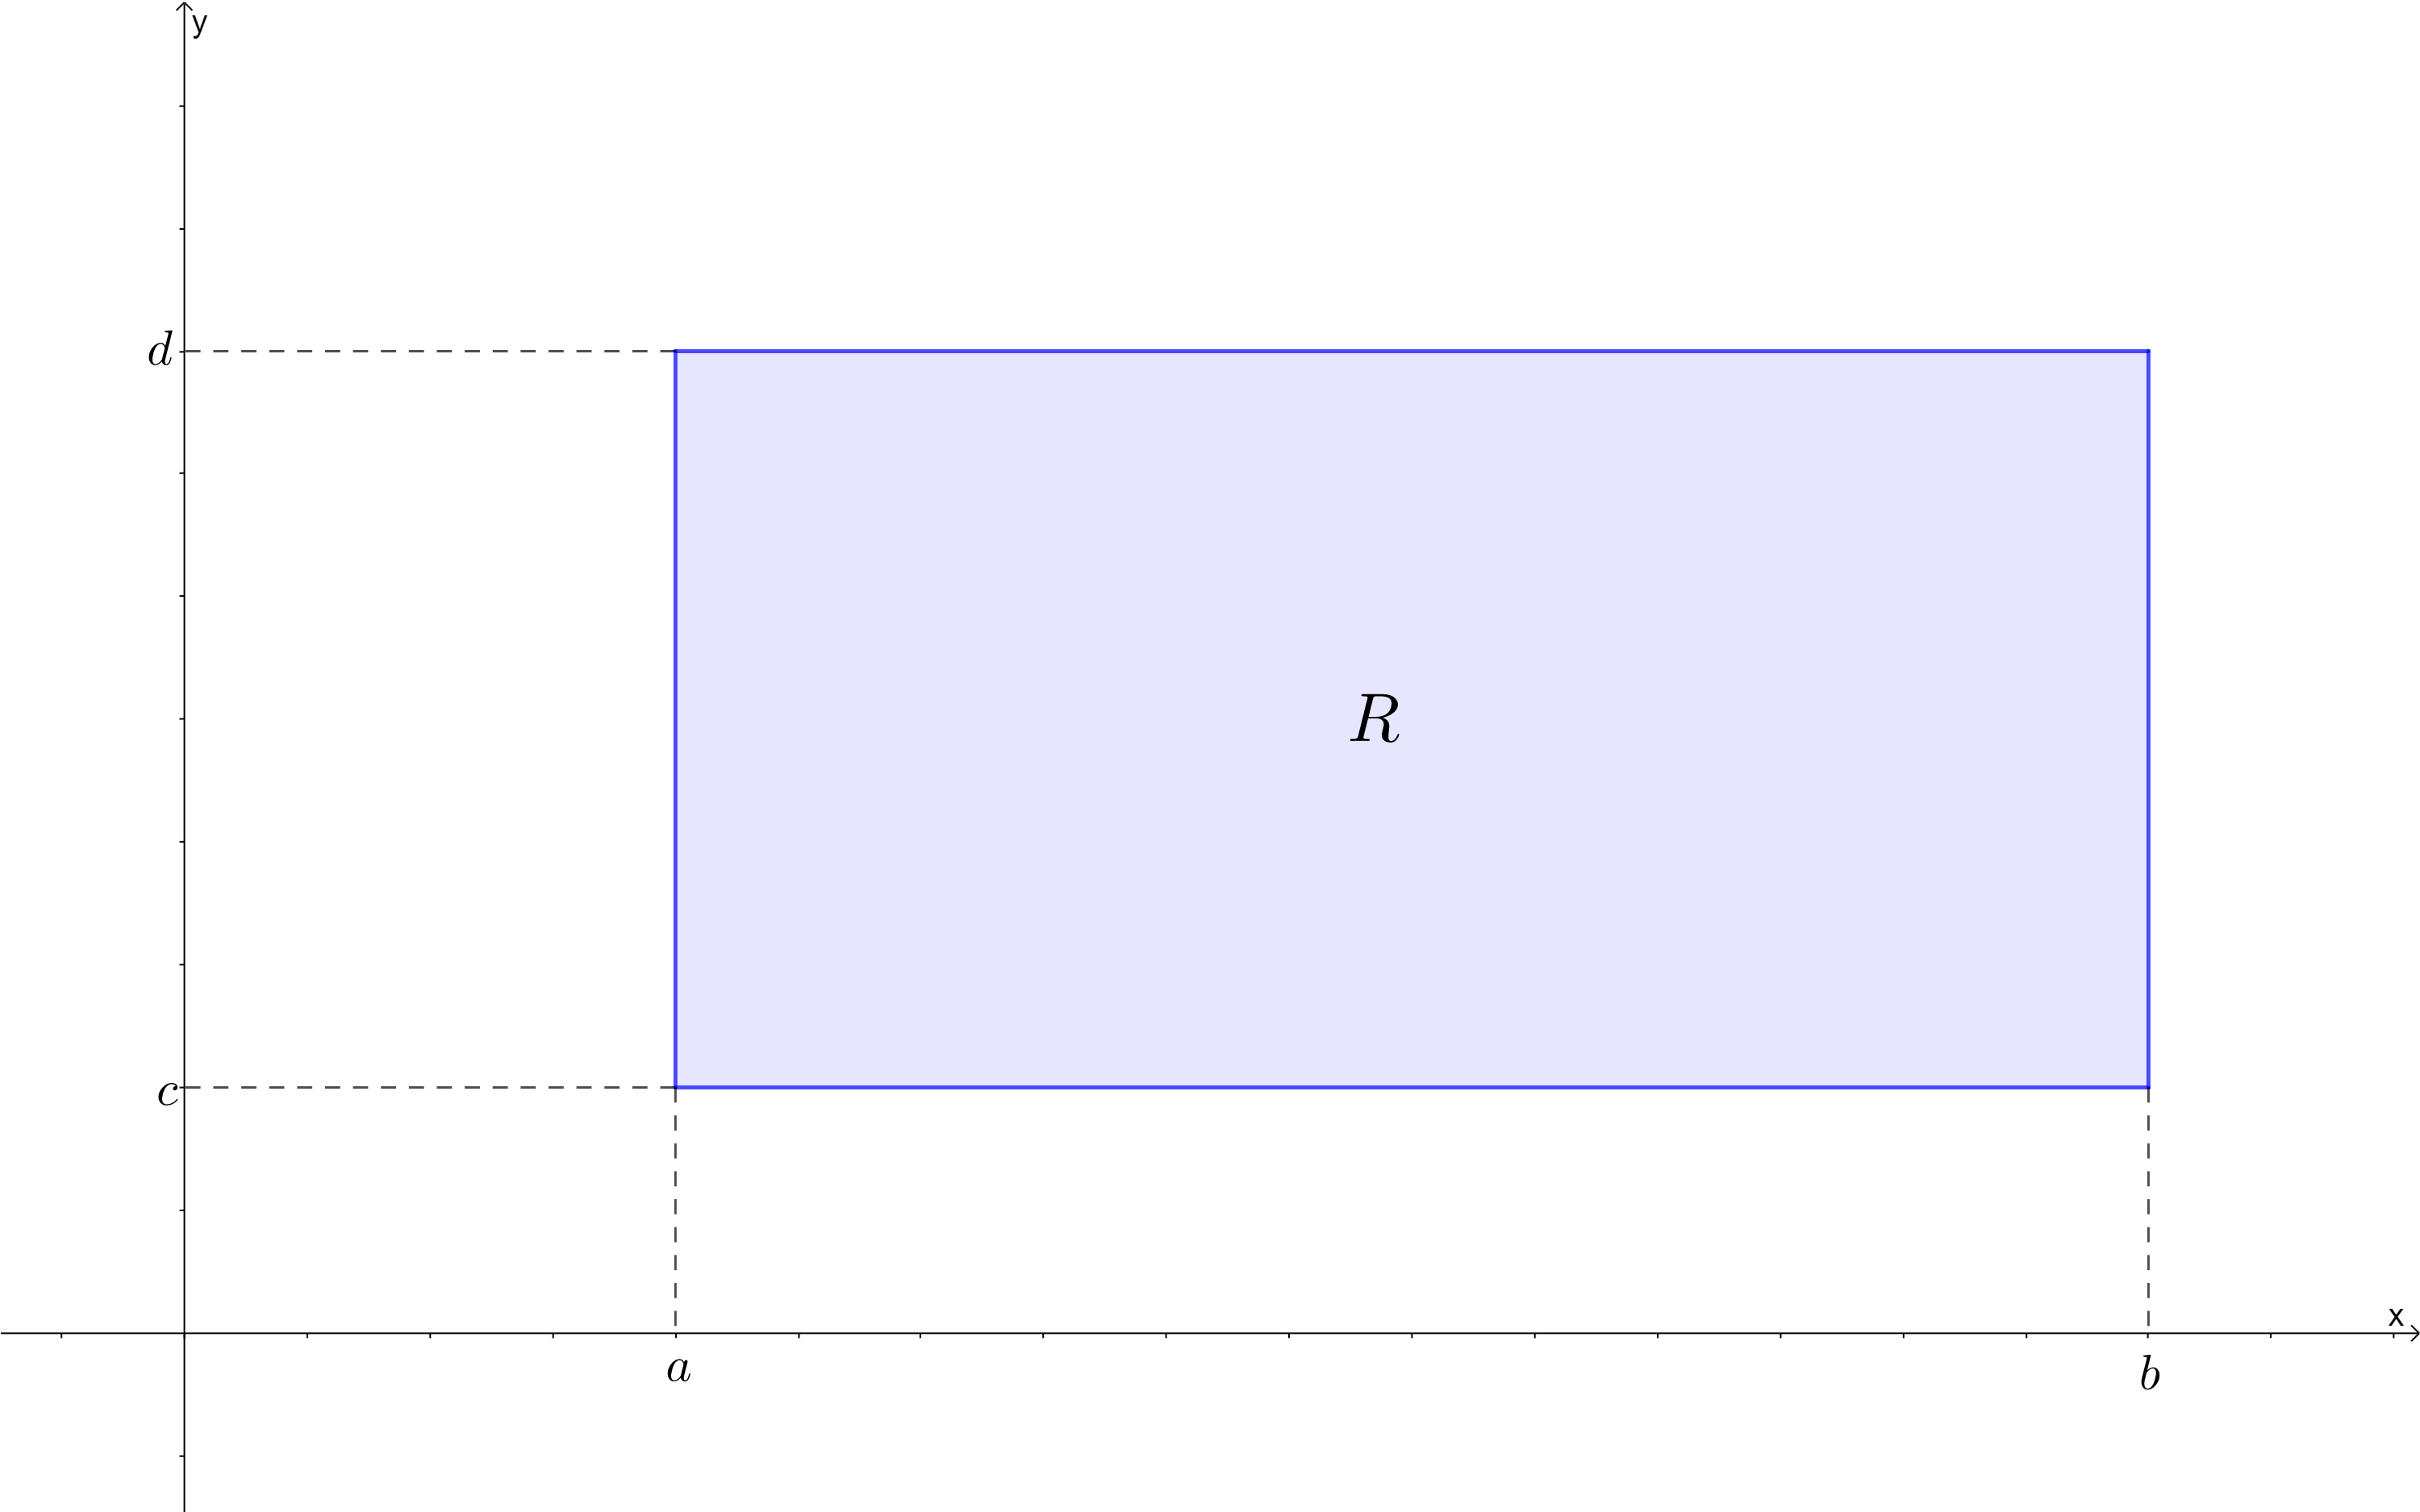
\includegraphics[scale=1.48]{Rbox.png}

$$\iint_R f(x,y)\, dA=\int_a^b \int_c^d f(x,y)\, dy\,dx = \int_c^d \int_a^b f(x,y)\, dx\,dy $$
\newpage
\subsubsection{Double Integrals Over General Domains}
\begin{enumerate}
\item \textbf{Type 1, Vertically Simple Region}: 

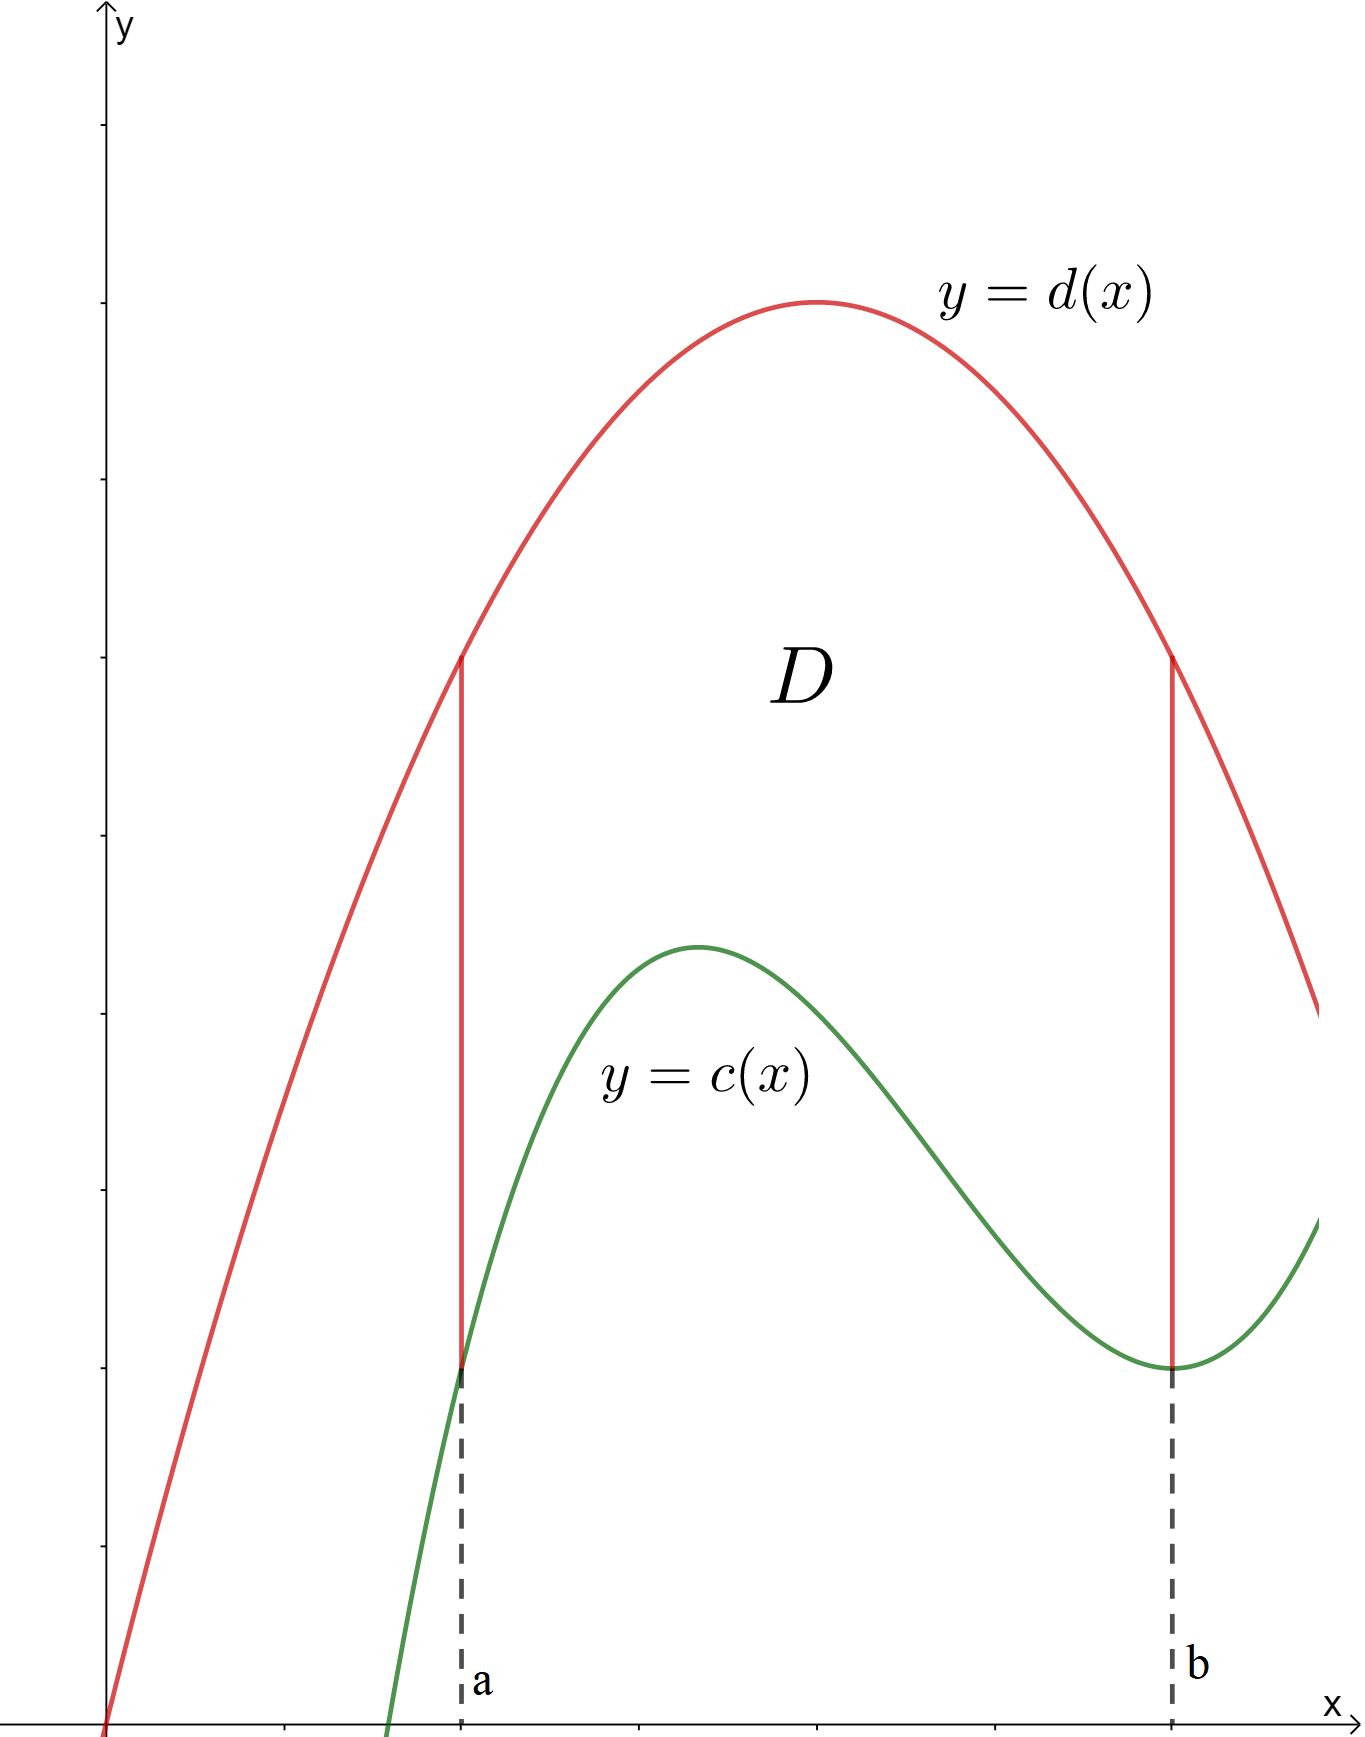
\includegraphics[scale=0.36]{ysimple.png}

$$\iint_D f(x,y) = \int_a^b \int_{c(x)}^{d(x)} f(x,y)\,dy\,dx$$
\newpage
\item \textbf{Type 2, Horizontally Simple Region}:

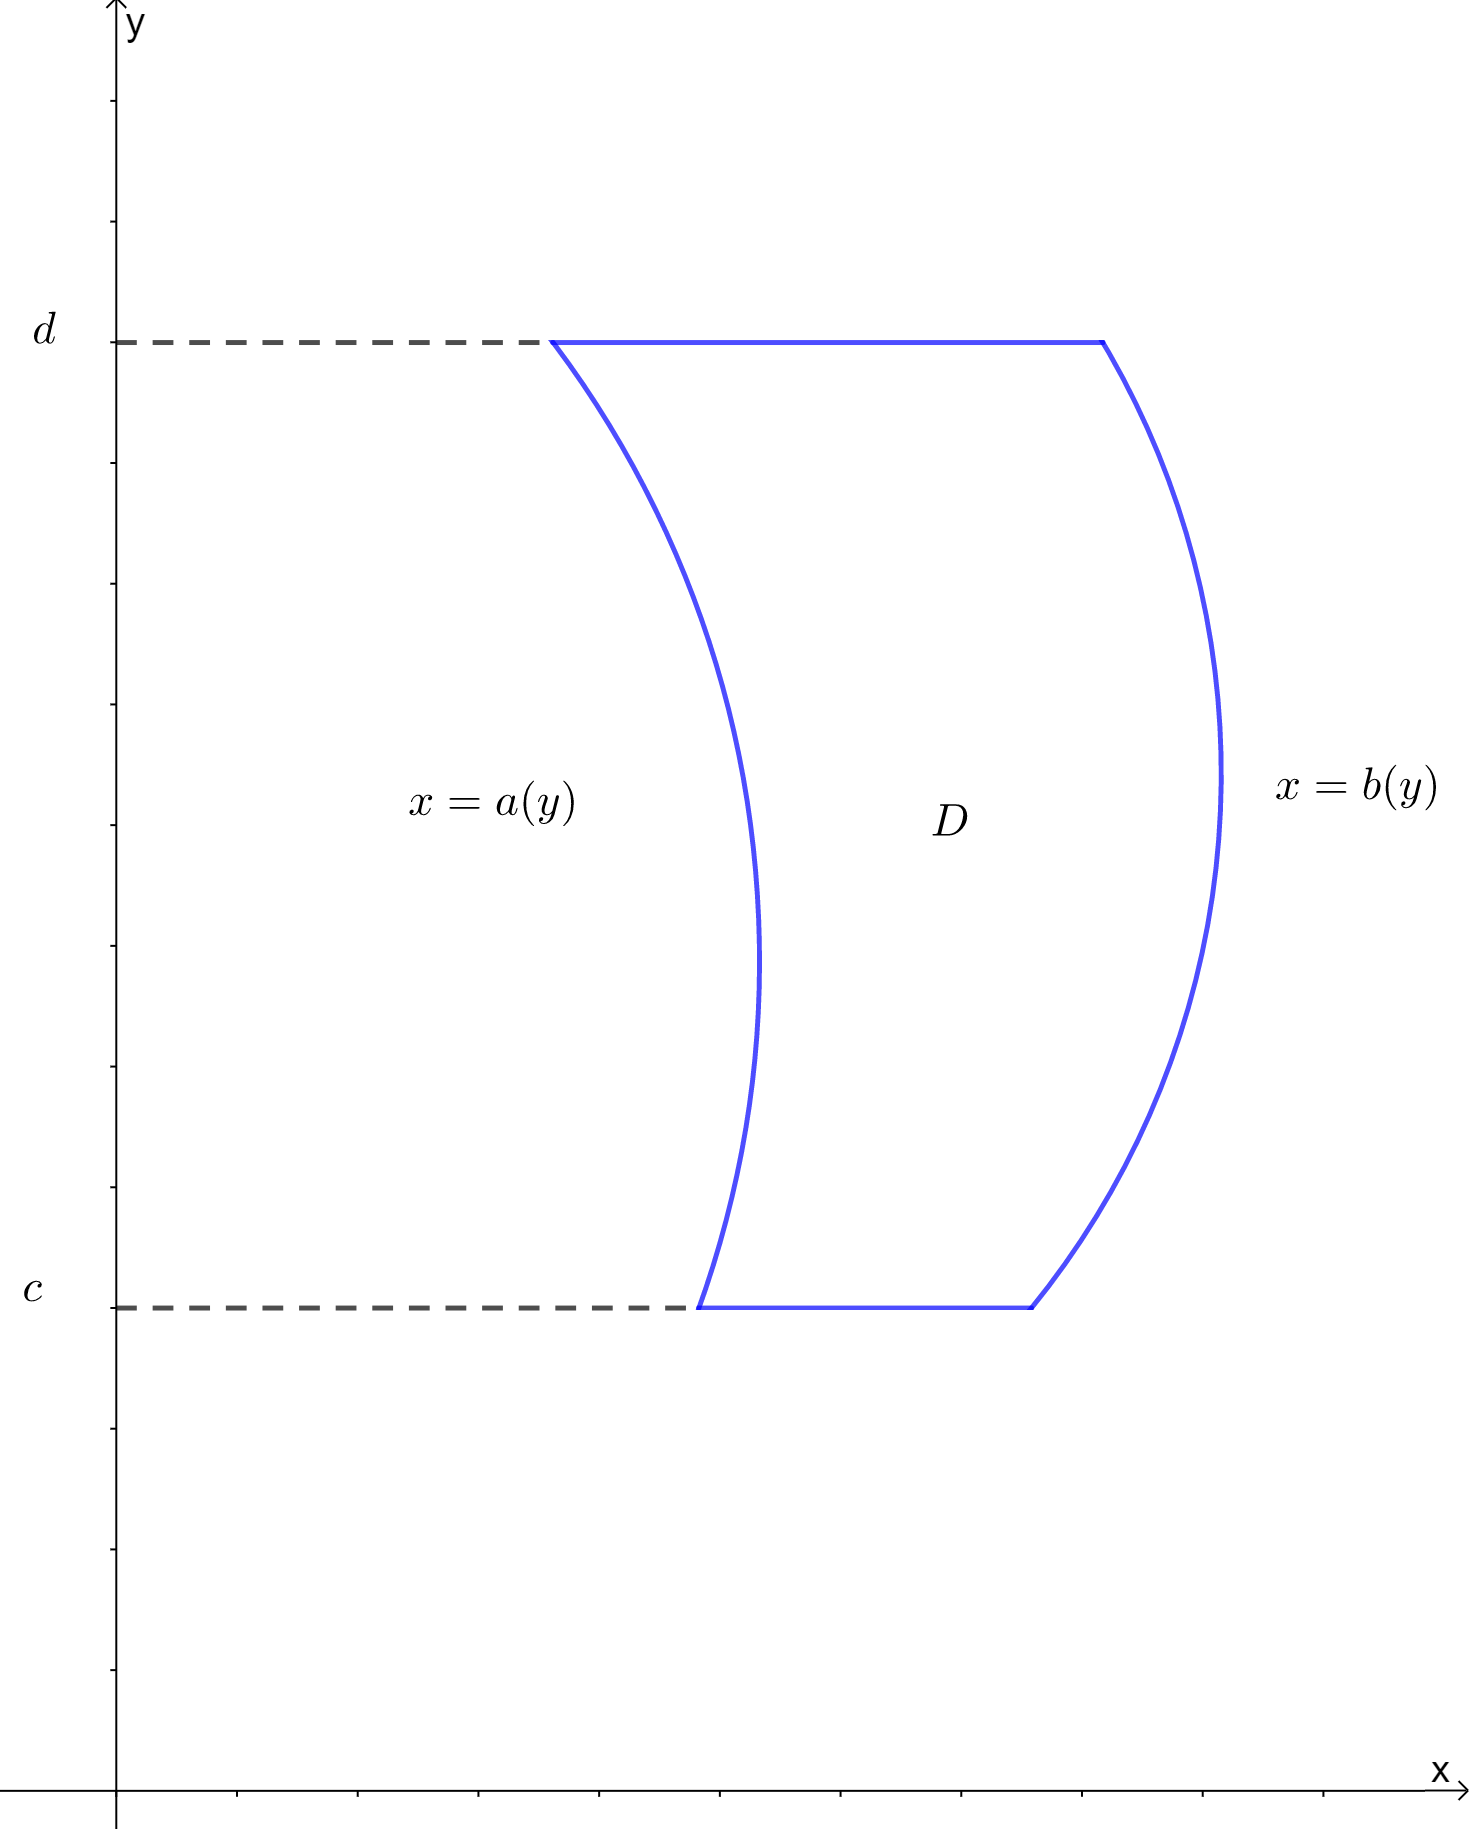
\includegraphics[scale=0.35]{xsimple.png}

$$\iint_D f(x,y) = \int_c^d \int_{a(y)}^{b(y)} f(x,y)\,dx\,dy$$

\end{enumerate}
If the regions are selected the difficult way, generally integrals can only be solved by multiple complementary integrals.

\subsubsection{Properties of Double Integrals}
\begin{enumerate}
\item $\displaystyle{\iint_D 1\, dA = }$ area of $D$.
\item $\displaystyle{\iint_D |f(x,y)|\,dA}$ = Volume of the solid lying vertically above $D$.

\end{enumerate}
\subsubsection{Double Integrals in Polar Coordinates}
$$x=r \cos \theta, y=r \sin \theta$$
$$r^2=x^2+y^2, \tan \theta = \frac{y}{x}$$
$$dA = dx\,dy = r\,dr\,d\theta$$
\subsection{Triple Integrals}
We have talked about horizontally and vertically simple regions for double integration. In triple integrals, we have three variables to iterate so there are 6 ways to formulate a triple integral. Again, all six ways are acceptable to formulate the iteration but being able to form the integral boundaries does not always imply that the integrals are simple solvable -or easy enough to solve-, there may be easier iteration orders and harder iteration orders.

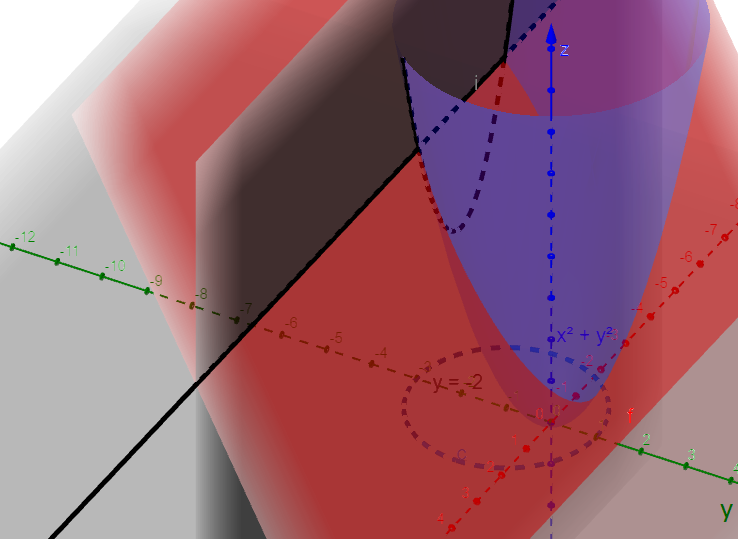
\includegraphics[scale=0.55]{ex1.png}

$$\int_{-3}^1 \int_{-\sqrt{4-(y+1)^2}}^{\sqrt{4-(y+1)^2}} \int_{x^2+y^2}^{3-2y} 1\,dz\,dx\,dy $$
\subsubsection{Properties of Triple Integrals}
\begin{enumerate}
\item $\displaystyle{\iiint_S 1\,dV}= $ volume of S. 
\end{enumerate}
\subsubsection{Triple Integrals over Cylindrical Coordinates}
$$x=r\cos \theta, \ \ y=r\sin \theta, \ \ z=z$$
$$r=\sqrt{x^2+y^2},\ \ \theta = \arctan \frac{y}{x}\ \ , z=z$$
$$dV=dx\,dy\,dz=r \,dr \,d\theta\, dz$$
\subsubsection{Triple Integrals over Spherical Coordinates}
$$x=R\sin\phi\cos\theta, y=R\sin\phi\sin\theta,z=R\cos\phi$$
$$R= \sqrt{x^2+y^2+z^2}\ \ , \theta = \arctan \frac{y}{x} \ \ , \phi = \arccos \left(\dfrac{z}{\sqrt{x^2+y^2+z^2}} \right)$$
$$dV=dx\,dy\,dz=R^2\sin\phi\,dR\,d\phi\,d\theta$$
Note: Some authors prefer $\rho$ instead of $R$.
\subsection{Surface Area}
Let $f$ be a function of two variables that is differentiable on $D$. The surface area of the graph of $f$ evaluated at $D$ is $$ S_f = \iint_D \sqrt{1+f^2_x+f^2_y} \,dA$$

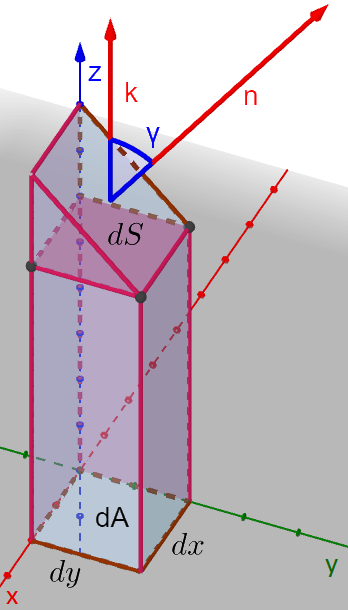
\includegraphics[scale=0.46]{surf.png}

\end{document}